%Modified from a template provided by Jennifer Pan, August 2011

\documentclass[10pt,letter]{article}
	% basic article document class
	% use percent signs to make comments to yourself -- they will not show up.
\usepackage{pdfsync}
\usepackage{amsmath}
\usepackage{amssymb}
\usepackage{amsthm}
	% packages that allow mathematical formatting

\usepackage{graphicx}
	% package that allows you to include graphics
\graphicspath{ {./images/} }

\usepackage{setspace}
	% package that allows you to change spacing

\onehalfspacing
	% text become 1.5 spaced

\usepackage{fullpage}
% package that specifies normal margins

\usepackage[parfill]{parskip}

\newtheorem*{thm}{Theorem}
\newtheorem{nthm}{Theorem}
\newtheorem{lem}{Lemma}

\begin{document}
	% line of code telling latex that your document is beginning

\title{Problem Set 2}

\author{Katherine Cheng, Richard Davis, Marty Keil}

% \date{Friday April 10, 2015}
	% Note: when you omit this command, the current date is automatically included
 
\maketitle 
	% tells latex to follow your header (e.g., title, author) commands.


\section*{Problem 1: Fibonacci Numbers}

\begin{thm}The sum of the squares of the first $n$ Fibonacci numbers is $F_{n}(F_{n+1})$\end{thm}
\begin{proof}
Let $P(n)$ be the statement ``the sum of the squares of the first $n$ Fibonacci numbers is $F_{n}(F_{n+1})$." We will prove, by induction, that $P(n)$ is true for all $n\geq1$, from which the theorem follows. 

\item For our base case, we need to show that P(0) is true, meaning that the sum of the squares of the first zero Fibonacci numbers is $F_{0}(F_{0+1})$. Since the sum of the first zero Fibonacci numbers is zero, and $F_{0}(F_{0+1})$ is zero as well, we see that $P(0)$ is true.

\item For the inductive step, assume that for some $k \in \mathbb{N} \geq 1$ that P(k) holds, meaning that:

\begin{equation} \label{eq:1}
0^2 + 1^2 + 1^2 + 2^2 + 3^2 + 5^2 ... F_{k}^2 = F_{k}(F_{k+1})
\end{equation}

\item We need to show that $P(k+1)$ holds, meaning that the sum of the squares of the first $k+1$ Fibonacci numbers is $F_{k+1}(F_{k+1+1}) = F_{k+1}(F_{k+2})$. To see this, notice that:
\begin{align*}
0^2 + 1^2 + 1^2 + 2^2 + 3^2 + 5^2 ... F_{k+1}^2 &= (0^2 + 1^2 + 1^2 + 2^2 + 3^2 + 5^2 ... F_{k}^2) + F_{k+1}^2\\
&= F_{k}(F_{k+1}) + F_{k+1}^2 \tag{via (1)}\\ 
&= F_{k}(F_{k+1}) + F_{k+1}(F_{k+1})\\
&= F_{k+1}(F_{k}+F_{k+1})\\
&= F_{k+1}(F_{k+2})\tag{via Fibonacci recurrence relation}
\end{align*}
Therefore, $P(k+1)$ is true, completing the induction. 
\end{proof}

\pagebreak

\section*{Problem 2: A Lot of Rocks?}

\begin{thm}No natural number of rocks is a lot of rocks\end{thm}
\begin{proof}
Let $P(n)$ be the statement that ``no natural number of rocks is a lot of rocks," where ``a lot of rocks" is defined as, ``a number of rocks that isn't zero and where if you remove one of the rocks, you're left with a lot of rocks." We will prove, by induction, that $P(n)$ is true for all $n \in N$, from which the theorem follows. 

\item For our base case, we need to show that P(0) is true, meaning that zero is not ``a lot of rocks". Since the definition of ``a lot of rocks" states that the number of rocks cannot be zero, we see that $P(0)$ is true.

\item For the inductive step, assume that for some $k \in \mathbb{N}$ that $P(k)$ holds, meaning that:
\begin{equation} \label{eq:2}
k \neq \mbox{a lot of rocks}
\end{equation}

\item We need to show that $P(k+1)$ holds, meaning that $k+1$ is not ``a lot of rocks". To see this, notice that:
\begin{align*}
n &= k+1\\
n-1 &= k+1-1 \tag{remove one rock}\\ 
&= k+(1-1)\\
&= k\\
&\neq \mbox{a lot of rocks} \tag{via (2)}
\end{align*}
Since the definition of ``a lot of rocks" states that ``if you remove one of the rocks, you're left with a lot of rocks," we conclude that $k+1$ is not ``a lot of rocks." Therefore, $P(k+1)$ is true, completing the induction. 
\end{proof}

\section*{Problem 3: Tiling with Triominoes}
\begin{thm}
  It is always possible to tile a grid of size $2^n \times 2^n$ that's missing exactly one square with right triominoes.
\end{thm}

\begin{proof}
By induction. Let $P(n)$ be ``it is always possible to tile a grid of size $2^n \times 2^n$ that's missing exactly one square (it doesn't matter which square) with right triominoes.'' We will prove that $P(n)$ is true for all natural numbers $n$. 

\textbf{P(0) base case - in case we decide to go with this one}

As our base case, we prove that $P(0)$ is true; that is, that it is possible to tile a grid of size $2^0 \times 2^0$ with any square missing with right triominoes. Since there is only one square in a $2^0 \times 2^0 = 1 \times 1$ grid, and the grid is missing exactly one square, it is trivially true that it is possible to tile the grid with right triominos.

\textbf{P(1) base case}

As our base case, we prove that $P(1)$ is true; that is, that it is possible to tile a grid of size $2^1 \times 2^1$ with any square missing with right triominoes. There are four possible squares in a $2 \times 2$ grid that can be missing: (a) top-left, (b) top-right, (c) bottom-right, (d) bottom-right. In each of these cases, we can place a single right triomino so that all the non-missing squares are covered (Figure \ref{fig:tile_base}).

\begin{figure}[h]
    \centering
    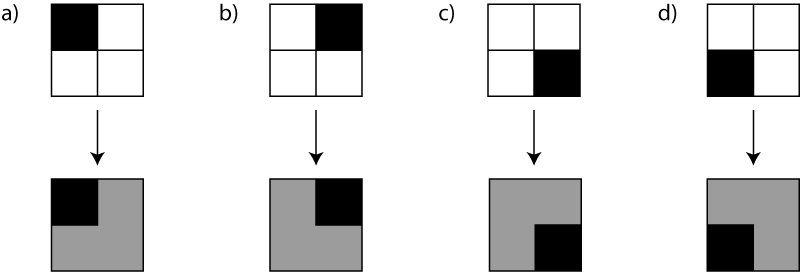
\includegraphics[width=0.8\textwidth]{rightTriominoes.png}
    \caption{Base Case, black square is missing}
    \label{fig:tile_base}
\end{figure}

For the inductive step, assume that for some $k \in \mathbb{N}$ that $P(k)$ is true. This means that it is possible to tile a $2^k \times 2^k$ grid with any square missing with right triominoes. We will prove that $P(k+1)$ is true, that it is possible to tile a $2^{k+1} \times 2^{k+1}$ grid with any square missing with right triominoes. 

Start with a $2^{k+1} \times 2^{k+1}$ grid with no squares missing, then remove a single square at any point in the grid. We will show that it is always possible to recreate this board by combining four $2^k \times 2^k$ boards with a single square missing in each. 

The larger board is made up of four quadrants, each of size $2^k \times 2^k$. The missing square must reside in one of these quadrants. From our inductive hypothesis we know that, taken alone, it is possible to tile this quadrant with right triominoes. 

What about the other three quadrants? Also from our inductive hypothesis, we know that it is possible to tile each of these with right triominoes as long as we remove a single square from each. It does not matter which square we remove. So, we remove a single square from the corner of each of these three quadrants.

We now have four separate $2^k \times 2^k$ grids, each with a single square missing and each tiled with right triominoes. We can now recombine these grids to recreate the $2^{k+1} \times 2^{k+1}$ grid. We leave the first grid (the one containing the original missing square) where it is and rotate the three grids (the ones with corner pieces missing) until the missing squares all come together in the center. These missing squares will always form a missing space that can be tiled with a right triomino (Figure \ref{fig:tile_proof}).

\begin{figure}[h]
    \centering
    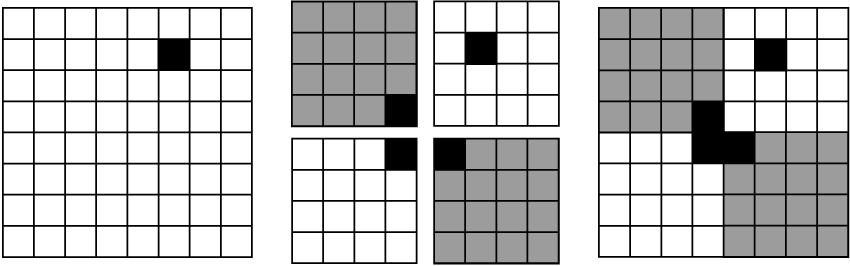
\includegraphics[width=0.8\textwidth]{rightTriominoesProof.png}
    \caption{Creating a $2^3 \times 2^3$ board from four $2^2 \times 2^2$ boards.}
    \label{fig:tile_proof}
\end{figure}

When that triomino is placed on the board, we will have successfully tiled the original $2^{k+1} \times 2^{k+1}$ board with a single square missing with right triominoes.

\end{proof}

\section*{Problem 4: The Circle Game}
Suppose that you have a circle with $2n$ arbitrary-chosen points on its circumfrence. $n$ of these points are labeled $+1$ and $n$ are labeled $-1$. Define this circle to be $C_n$. You can play a game where you choose one of these points as your starting point and then start moving clockwise around $C_n$. As you go, you'll pass through some number of $+1$ points and some number of $-1$ points. You lose the game if at any point in your journey you pass through more $-1$ points than $+1$ points. You win the game if you get all the way around to your starting point without losing.\\
\begin{nthm} \label{thm:circlethm}
  For any $n \in \mathbb{N}$ where $n \ge 1$, no matter which of the $n$ points are labeled $+1$ and which are labeled $-1$, there is always one point you can start at to win the game.
\end{nthm}

\begin{proof}
By induction. To prove this we will need two additional lemmas.
\begin{lem} \label{lemma:circle1}
For any $n \ge 1$, there is always at least one $(+1, -1)$ clockwise point pair on $C_n$.
\end{lem}
\begin{proof}
By induction. Let $Q(n)$ be ``you will always pass through a $(+1, -1)$ point pair while moving clockwise along $C_n$.'' We will prove that this holds for $Q(n+1)$.

As our base case, we prove that $Q(1)$ is true. $C_1$ is a circle with a single $+1$ point and a single $-1$ point. We see that there is, indeed, a $(+1, -1)$ clockwise point pair on this circle.

For the inductive step, assume that for some $k \in \mathbb{N}$ that $Q(k)$ is true. This means that there is at least one $(+1, -1)$ point pair on $C_k$. We will use this to prove that $Q(k+1)$ is true, that there is at least one $(+1, -1)$ clockwise point pair on $C_{k+1}$. 

We can create $C_{k+1}$ by adding a $+1$ point and a $-1$ point anywhere on $C_k$. It is impossible to place either of these points in a way that eliminates the presence of the $(+1, -1)$ clockwise point pair that already exists on $C_k$. If we place the $+1$ between the existing $(+1, -1)$ pair, we create a new sequence $(+1, +1, -1)$ that still contains a $(+1, -1)$ clockwise point pair. If we place the $-1$ point between the existing $(+1, -1)$ pair, we create a new sequence $(+1, -1, -1)$ that still contains a $(+1, -1)$ clockwise point pair.
\end{proof}

\begin{lem} \label{lemma:circle2}
If a $(+1, -1)$ point pair is added into a winning path, the path remains a winning path.
\end{lem}

\begin{proof}
A winning path is defined as a path that never takes you through more $-1$ points than $+1$ points at any point in the journey. In other words, at any point the count of $+1$ points passed through, $p$, must be $\ge$ the count of $-1$ points passed through, $n$, or $p \ge n$. If we insert a $(+1, -1)$ clockwise point pair after any arbitrary point in a winning path and this inequality still holds at all points on the path, we will have shown that we can always insert a $(+1, -1)$ clockwise point pair into a winning path and it will remain a winning path. 

We insert a $(+1, -1)$ clockwise point pair into a winning path. No matter where we insert this, the inequality $p \ge n$ must hold at the point directly preceding the inserted pair. Passing through the first point in the $(+1, -1)$ clockwise point pair yields $(p+1) \ge n$. Passing through the second point in the $(+1, -1)$ clockwise point pair yields $(p+1) \ge (n+1)$. Since the original path was a winning path, $p \ge n$ is true, so $(p+1) \ge n$ and $(p+1) \ge (n+1)$ must also be true.

Thus, if a $(+1, -1)$ point pair is added into a winning path, the path remains a winning path.
\end{proof}

Now we can proceed with the proof of theorem \ref{thm:circlethm}. Let $P(n)$ be ``For any $n \in \mathbb{N}$ where $n \ge 1$, no matter which of the $n$ points are labeled $+1$ and which are labeled $-1$, there is always one point you can start at to win the game.'' We will prove that $P(n)$ is true for all $n \ge 1$.

As our base case, we prove that $P(1)$ is true. Because $C_1$ only has a single $+1$ point and a single $-1$ point, we immediately see that by starting at the $+1$ point we can win the game.

For the inductive step, assume that for some $k \in \mathbb{N}$ that $P(k)$ is true, meaning there is a point you can start at on circle $C_k$ to win the game. Let's start with $C_{k+1}$, a circle with $k+1$ positive points and $k+1$ negtive points. By lemma \ref{lemma:circle1}, we know that there is at least one $(+1, -1)$ clockwise point pair on $C_{k+1}$. If we remove this pair we are left with a new circle $C_k$. From our inductive hypothesis, we know that there is at least one winning path on this circle. By lemma \ref{lemma:circle2}, we know that we can insert a $(+1, -1)$ clockwise point pair anywhere into this winning path and still have a winning path. This means we can insert the previously-removed $(+1, -1)$ clockwise point pair back into its original spot and the winning path will remain a winning path. This proves that there is at least one winning path in $C_{k+1}$. 
\end{proof}

\section*{Problem 5: Binomial Trees}
Binomial trees are a specific family of directed trees defined as follows: a binomial tree of order $n$ is a single node with $n$ children, which are binomial trees of order $0, 1, 2, \ldots, n-1$. 

\begin{thm}
A binomial tree of order $n$ has exactly $2^n$ nodes.
\end{thm}

\begin{proof}
By strong induction. Let $P(n)$ be ``a binomial tree of order $n$ has exactly $2^n$ nodes.'' We will prove that $P(n)$ holds for all natural numbers $n$. 

As our base case, we will prove that $P(0)$ is true. A binomial tree of order 0 is a single node with no child nodes. Because $1 = 2^0$ we show that our base case is true.

For the inductive step, assume that for some $n \in \mathbb{N}$, that for any $k \le n$, that $P(k)$ holds and that a binomial tree of order $k$ has exactly $2^k$ nodes. 

By definition, we know that a binomial tree of order $k+1$ has $k+1$ children, which are themselves binomial trees of order $0, 1, 2, \ldots, k$ (see figure \ref{fig:binTree}).

\begin{figure}[h]
    \centering
    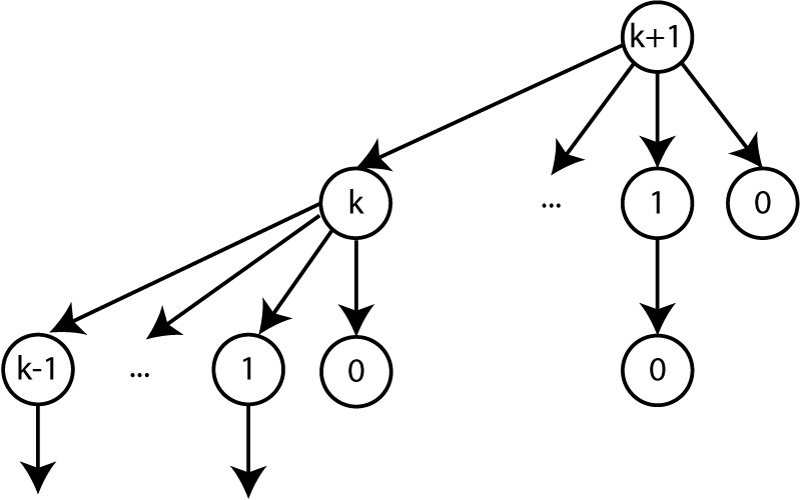
\includegraphics[width=0.5\textwidth]{binTree.png}
    \caption{Binomial tree of order $k+1$}
    \label{fig:binTree}
\end{figure}

To find the total number of nodes in a binomial tree of order $k+1$ we need to add all of the nodes of the children plus one for the root node. By the inductive hypothesis we know that each of the children trees have $2^0, 2^1, 2^2, \ldots, 2^k$ nodes. Thus, the total number of nodes in the binomial tree of order $k+1$ is given by 
\begin{equation} \label{eq:bintree}
1 + \sum_{i=0}^{k} 2^i.
\end{equation} 
In page 102 of the Mathematical Foundations of Computing course reader it is proved that 
\begin{equation*}
\sum_{i=0}^{j-1} 2^i = 2^j - 1.
\end{equation*} 
Letting $j = k+1$ gives us 
\begin{equation*}
\sum_{i=0}^{k+1-1} 2^i = 2^{k+1} - 1
\end{equation*} 
Plugging this into \ref{eq:bintree} gives us
\begin{equation*}
1 + (2^{k+1} - 1) = 2^{k+1}
\end{equation*}
Therefore, we have shown that a binomial tree of order n has exactly $2n$ nodes.
\end{proof}

\section*{Problem 6: Nim}
\begin{thm}
If the game of Nim  is played with just two piles of stones, each of which begins with exactly the same number of stones, then the second player can always win the game. 
\end{thm}
\begin{proof}
Let P(n) be the statement ``In every game which begins with two stone piles and with the exact same number of stones, n, the second player can always win." We will prove by induction that P(n) is true for all n $\geq$ 1, from which the theorem follows.

As a base case, we prove P(1), with two piles of 1 rock each the second player can always win. Player 1 must remove at least one rock and cannot remove rocks from more than one pile. Therefore, Player 1 will empty one pile. Player 2 can then always empty pile 2, leaving Player 1 with all empty piles. Player 2 then wins the game. 

For the inductive step, we assume there are there are k  $\in \mathbb{N}$ that P(1), P(2),..., P(k) are all true. In other words, we assume that in any game with k rocks in each pile at the beginning, player 2 can always win. We'll prove that for P(k+1), when there are k+1 rocks in each pile at the start, player 2 can always win as well . 

Since P(k) represents a pile with k rocks in each pile, P(k+1) means that one more rock has been added to each pile. Player 2 can always win in this game by removing the same number of rocks as Player 1, but from the opposite pile, for every turn. Take two possible cases using this strategy:

\textbf{Case 1:} Player 1 removes all k+1 rocks from one pile. Player 2 can then remove all k+1 rocks from the other pile. Player 1 is then left with two empty piles, therefore Player 2 can always win. 

\textbf{Case 2:} Player 1 removes some number of rocks between 1 and k from the pile. Player 2 removes the same number of rocks from the other pile. Both rock piles are now equal and there are between 1 and k rocks in each. 
From our inductive hypothesis we can then conclude that player 2 can always win this game. 

Since Player 2 can always win in both cases when there are k+1 rocks in each pile, P(k+1) is true, completing the induction. 
\end{proof}

\section*{Problem 7: Tournament Winners}
\begin{thm}
Every tournament with at least one player has a tournament winner. 
\end{thm}
\begin{proof}
Let P(n) be the statement ``every tournament with n players has a tournament winner." We will prove by induction that P(n) is true for all n $\in \mathbb{N} \geq$ 1, from which the theorem follows.

As a base case, we prove P(1), that any tournament with one player has a tournament winner. In a tournament with just one player, this player does not play against anyone else, and therefore accumulates only wins, making it vacuously true that he will be the tournament winner. 

For the inductive step, we assume there are k  $\in \mathbb{N}$ that P(1), P(2),..., P(k) are all true. In other words, we assume that any tournament with at most k players has a tournament winner. We'll prove P(k+1), that any tournament with k+1 players has a tournament winner. 

Consider any tournament T with k+1 players. Choose any one player p and form two sub-tournaments, a sub tournament $T_0$ of all the players who beat p and a sub tournament $T_1$ of all the players p beat. Both of these sub-tournaments has from 0 to k players. Now we will split this problem into two possible cases. 

\textbf{Case 1:} $T_0$ has 0 players. If this the case then player p has beaten every other player in the tournament($T_1$), and is therefore the tournament winner for tournament T, since there are no other players remaining in the tournament.  

\textbf{Case 2:} $T_0$ has at least one player. If this is the case, then by our inductive hypothesis, $T_0$ has a tournament winner W. W, like all members of $T_0$, has beaten p. Since p has beaten all of T's remaining players in $T_1$, W is also the tournament winner for tournament T. 

Therefore, since there is a tournament winner in both cases of this arbitrary tournament of k+1 players, P(k+1) is true, completing the induction. 

\end{proof}

% \section*{Appendix: Referencing Equations}
% \begin{equation} \label{eq:divbyzero}
%   \frac {1} {0}
% \end{equation}

% This references \ref{eq:divbyzero}.

\end{document}
	% line of code telling latex that your document is ending. If you leave this out, you'll get an error

%%% Local Variables:
%%% mode: latex
%%% TeX-master: t
%%% End:
